\documentclass[11pt]{article}
\usepackage{../shared/hanzocover}
\usepackage[utf8]{inputenc}
\usepackage[T1]{fontenc}
\usepackage{amsmath,amssymb}
\usepackage{graphicx}
\usepackage{booktabs}
\usepackage{multirow}
\usepackage{array}
\usepackage{enumitem}
\usepackage{xcolor}
\usepackage{tikz}
\usetikzlibrary{shapes,arrows.meta,positioning,fit,backgrounds,calc}
\usepackage{pgfplots}
\pgfplotsset{compat=1.18}
\usepackage[hidelinks]{hyperref}

\definecolor{hzblue}{rgb}{0.12,0.30,0.55}
\definecolor{hzslate}{rgb}{0.22,0.25,0.30}
\definecolor{hzgreen}{rgb}{0.10,0.45,0.25}
\definecolor{hzred}{rgb}{0.60,0.16,0.16}

\newcommand{\arm}[1]{\texttt{#1}}

\title{Retrieval Scoped by Subject\\[0.35em]
{\large A factorial measurement of conversational memory on LoCoMo,\\
and the negative controls that locate the effect}}
\author{
    Hanzo AI Research\thanks{Corresponding author: research@hanzo.ai} \\
    \textit{Hanzo Industries Inc (Techstars '17)} \\
    Los Angeles, California \\
    \texttt{https://hanzo.ai}
}
\date{Measurement pass 2026-09-09 \quad \texttt{hanzoai/semantic} v0.2.4}

\begin{document}

\hanzocoverpage
\maketitle

\begin{abstract}
\noindent
We measure a graph-structured conversational memory against a flat
nearest-neighbour index on LoCoMo~\cite{locomo} --- 10 conversations, 272
sessions, 5{,}882 turns, 1{,}986 questions --- using the benchmark's own
scorer, ported and verified against the original Python on all 1{,}986
questions and every system reported here. Three results follow, and the negative
controls are the substance of the paper.

First, the aggregate over all five question categories is degenerate. A system
that replies ``No information available'' to every question scores $0.228$,
above every system here that has to find its own evidence; only an oracle
handed the dataset's own annotated evidence scores higher, at $0.252$. A
quarter of LoCoMo's questions are adversarial and the official metric awards a
point for declining them, so any mean over the full set measures the abstention
rate before it measures the memory. The answerable and adversarial halves have
to be reported apart.

Second, the effect that survives is subject scope. Restricting retrieval to
the person a question names scores $0.502$ against $0.200$ on the 446
adversarial questions (95\% CI over conversations $[+0.247, +0.347]$) at no
measurable cost on the 1{,}540 answerable ones ($0.142$ against $0.144$, CI
$[-0.010, +0.006]$). The mechanism is reader-independent: with the result limit
lifted past the size of the conversation, the graph memory can reach $76\%$ of
the annotated evidence for answerable questions and $27\%$ for adversarial ones,
where the flat index reaches $99\%$ and $96\%$. It is selectively blind, and
the blindness falls where the trap turns are. Abstention is the variable this
runs through: the flat index's retrieval confidence separates answerable from
adversarial questions at AUC $0.514$, which is chance; the graph memory's
separates them at $0.698$.

Third, the controls remove most of the explanation the system's name suggests.
Emptying the knowledge graph entirely leaves every reported figure
byte-identical --- retrieval never consults it. Deleting the inference step,
which derived 44 facts from 23{,}942 extracted claims, moves no score on either
half and no figure anywhere by more than two thousandths. A $2\times2$ over what is indexed against what a query may reach
attributes $+0.152$ of the adversarial gain to subject scope applied to the
unchanged turn index, $-0.029$ to the claim-span unit applied on its own, and
$+0.179$ to their interaction. An oracle handed
the dataset's own annotated evidence scores \emph{worse} on adversarial
questions than the graph memory does ($0.426$ against $0.502$), because on those
questions the trap turn is the annotated evidence.

No language model was called, in either index or the reader, so absolute F1 is
far below published model results on this benchmark and is not comparable to
them; the systems are comparable to each other because they differ in exactly
one thing at a time. The harness is public, stdlib-only, and fetches the
dataset itself.
\end{abstract}

\tableofcontents
\vspace{1em}

\section{Introduction}
\label{sec:intro}

A conversational agent that has spoken with someone for months is asked a
question today about something said in March. The store it searches holds
thousands of turns across dozens of sessions. Some of the questions it will be
asked have no answer in that store at all, and answering them anyway is the
failure that users notice.

The default construction is a nearest-neighbour index over turns: embed each
turn, embed the question, return the closest few, and let a reader compose an
answer from them~\cite{rag,dpr}. Its failure on a long conversation is specific.
A turn near the question's words is not the same thing as a turn about the
person the question names, and in a two-party conversation held over months
those two criteria come apart constantly, because both speakers discuss the
same topics. The remedy usually proposed is structure: extract entities and
relations, build a graph across sessions, and retrieve through
it~\cite{graphrag,hipporag}. Our own earlier measurement on this
corpus~\cite{multihop} ended by naming that structure as the missing signal.

This paper tests that proposal and reports what actually carries the result. We
built the graph memory --- read every turn for who did what, fold the claims
into a graph so that a person mentioned in two sessions is one node, close the
graph under an inference rule, index what each person said in each turn, and
answer by looking up the person a question names --- and ran it against a flat
turn index over the same conversations, the same term weighting, the same
reader, and the same scorer.

The headline comparison favours the graph. The controls say why, and the why is
smaller and more specific than the construction:

\begin{itemize}[leftmargin=1.2em,itemsep=2pt]
\item The aggregate that would usually be quoted is arithmetic, not a result
      (\S\ref{sec:degenerate}).
\item The graph itself is inert. Emptying it changes nothing
      (\S\ref{sec:control-graph}).
\item The inference step is inert. Removing it moves no score on either half
      (\S\ref{sec:control-reason}).
\item What remains is a partition of the index by the subject of a sentence and
      a filter on the query, and a $2\times2$ locates the effect there
      (\S\ref{sec:factorial}).
\end{itemize}

\paragraph{Status of the claims.} Sections
\ref{sec:degenerate}--\ref{sec:where-not} are measurements produced by the
harness described in \S\ref{sec:repro}; every number in them is reproducible
from a public repository and a public dataset. Section~\ref{sec:mechanism}
combines measurement with an interpretation of it, and says which sentence is
which. Sections~\ref{sec:limits} and \ref{sec:settle} are limitations and
proposed experiments, and are not evidence for anything.

\section{Setup}
\label{sec:setup}

\subsection{The corpus}

LoCoMo~\cite{locomo} is ten synthetic two-party conversations, generated to
span months and then human-verified, with per-question annotations naming the
turns that constitute the evidence. We use the released \texttt{locomo10.json}:
272 sessions, 5{,}882 turns, 1{,}986 questions. The questions are typed, and the
types are scored differently:

\begin{center}
\small
\begin{tabular}{@{}llr@{}}
\toprule
category & what it asks & $n$ \\
\midrule
single hop  & one turn holds the answer              & 841 \\
multi hop   & several turns, usually several sessions & 282 \\
temporal    & when something happened                 & 321 \\
open domain & an inference beyond what was said       & 96 \\
adversarial & a question with no answer in the conversation & 446 \\
\midrule
answerable  & the first four, together               & 1{,}540 \\
\bottomrule
\end{tabular}
\end{center}

The adversarial category is the one that structures this paper. Its questions
are not nonsense and not out-of-domain. They are questions about the wrong
person: an activity that speaker~A described is attributed to speaker~B, who
was present, asked about it, and never claimed it. Only two of the 446 carry a
reference answer at all. The rest carry a field \texttt{adversarial\_answer}
holding the plausible wrong one --- for the worked example of
\S\ref{sec:result} it is literally \emph{yoga} --- and the scorer reads neither
field (\S\ref{sec:metric}). What makes a reply right on this category is that it
declines. LoCoMo's construction here follows the
unanswerable-question design of SQuAD~2.0~\cite{squad2}, where a plausible
distractor is present in the passage and the correct response is abstention.

\subsection{The metric}
\label{sec:metric}

We use the benchmark's own scorer, \texttt{task\_eval/evaluation.py}, and did
not write one. It normalises and stems both sides and compares them as token
bags, per category:

\begin{itemize}[leftmargin=1.2em,itemsep=1pt]
\item single hop and temporal: token-level F1 against the reference;
\item open domain: F1 against the first of several accepted phrasings;
\item multi hop: both sides split on commas, each reference part scored against
      its best-matching reply part, so recall is rewarded and a wrong extra
      part costs nothing;
\item adversarial: one point if the reply contains ``no information available''
      or ``not mentioned''. \emph{The reference answer is not consulted.}
\end{itemize}

That last rule is not a detail. On a quarter of the benchmark the metric scores
a policy, not an answer, and \S\ref{sec:degenerate} is the consequence.

The harness is written in Go, so the scorer and the NLTK Porter
stemmer~\cite{porter,nltk} it calls were ported. The port is held against the
original three ways --- the stem of all 6{,}597 words in the corpus, the
normalisation of all 10{,}382 distinct questions, answers and turns, and the
score of 2{,}400 replies spanning every category and every branch --- and then
end to end: the original Python is run over the same predictions file the Go
writes. Every figure in Tables~\ref{tab:main} and \ref{tab:factorial} agrees
between the two to three decimals, across 1{,}986 questions and all six systems.
That end-to-end run needs one adaptation, which lives in our script and not in
the vendored file: the official recall reads the first retrieved identifier to
tell a session id from a dialogue id, and a memory that returned nothing has no
first identifier, so a placeholder matching no evidence is substituted for it.
Without the substitution the official code awards recall $1.0$ to a system that
returned nothing. The original scorer is fetched at test time rather than
vendored, because LoCoMo is CC BY-NC 4.0 and our repository is MIT.

We report three quantities throughout. \textbf{F1} is the official metric above.
\textbf{Reach} is the share of a question's annotated evidence turns the index
returned; it is a property of retrieval alone and owes nothing to the reader.
\textbf{Silence} is how often a system declined to answer. A difference between
two systems is computed from the unrounded per-question scores and rounded
once, so it need not equal the difference of the two rounded figures printed in
a table.

\subsection{The reader, and the ceiling it imposes}
\label{sec:reader}

No language model is called anywhere in this work. The reader is deterministic
and extractive: it takes the sentence covering most of the question's terms,
drops the words the question already contained, keeps the rarest few of what is
left, and for a \emph{when} question reads a date off the session, resolving a
month named in the text against it. It declines when the retrieved evidence
covers less than \texttt{floor} of the question's inverse-frequency-weighted
terms. It never sees the question's category and never sees which index
produced its evidence.

This choice caps the whole study, and the cap is measured rather than assumed.
The \arm{oracle} system in every table is handed exactly the turns the dataset
annotates as the evidence --- perfect retrieval, everything else unchanged. It
scores $0.202$ on the answerable questions at the operating point of
Table~\ref{tab:main} and $0.306$ with abstention turned off. So
$0.306$ is what perfect retrieval is worth through this reader, and the
distance from there to $1.0$ is the reader's alone. Two consequences follow and
we hold to both:

\begin{enumerate}[leftmargin=1.4em,itemsep=2pt]
\item Absolute F1 here is far below published results that use a model reader
      on this benchmark, and \textbf{is not comparable to them}.
\item The answerable column is nearly insensitive to retrieval quality: an
      index that reaches $99\%$ of the evidence and one that reaches $76\%$
      score $0.144$ and $0.142$ through this reader. Any claim of the form
      ``no cost on answerable questions'' is therefore a claim about what this
      reader can detect, and \S\ref{sec:limits} says so again.
\end{enumerate}

The reader's other settings do not matter much. Swept over all ten
conversations, the span of words it may take moves \arm{graph}'s overall
score from $0.215$ to $0.224$, the band within which a second piece of evidence
counts moves it from $0.220$ to $0.223$, and the number of pieces from $0.220$
to $0.223$. The two settings that do matter, the result limit $k$ and the
abstention floor, both trade answering against declining, and both are swept in
\S\ref{sec:abstention}.

\subsection{Four indexes, as a factorial}
\label{sec:indexes}

The graph memory differs from a flat turn index in two ways at once. It indexes
a narrower unit --- what one person said in one turn, which we call a
\emph{claim span} --- and it restricts what a query may reach to the pieces
belonging to the \emph{subject} of the question, the person the question names.
Two systems cannot separate two factors, so we built all four cells
(Figure~\ref{fig:design}):

\begin{center}
\small
\begin{tabular}{@{}lll@{}}
\toprule
system & indexed unit & reachable \\
\midrule
\arm{vector} & whole turn & everything \\
\arm{scoped} & whole turn & the subject's turns only \\
\arm{span}   & claim span & everything \\
\arm{graph}  & claim span & the subject's spans only \\
\bottomrule
\end{tabular}
\end{center}

Every cell ranks by cosine over the same inverse-frequency-weighted stemmed
terms, through the same in-memory store, with the same $k$, read by the same
reader and marked by the same scorer. The subject restriction is a metadata
filter on the query, not a second store. The comparison is therefore an
ablation of one index, not a comparison of two systems.

\begin{figure}[t]
\centering
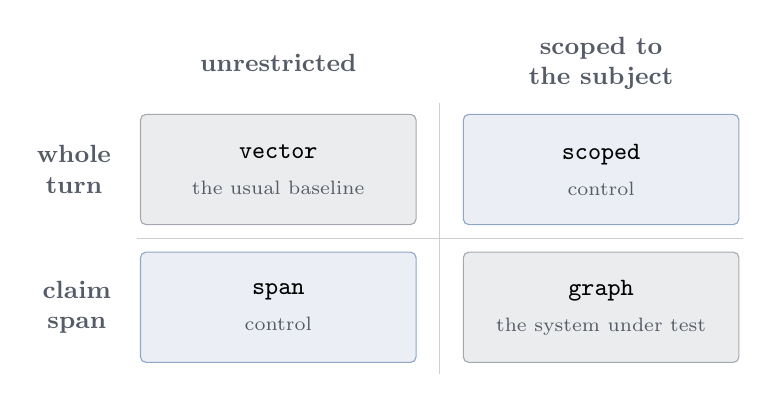
\begin{tikzpicture}[
  font=\small,
  cell/.style={draw=hzslate!45, rounded corners=2pt, minimum width=35mm,
               minimum height=14mm, align=center, inner sep=2pt},
  base/.style={cell, fill=hzslate!10},
  new/.style={cell, fill=hzblue!9, draw=hzblue!50},
  hd/.style={hzslate!85, font=\small\bfseries, align=center}
]
\newcommand{\gloss}[1]{{\scriptsize\color{hzslate!85}#1}}

\node[hd] at (2.05, 1.35) {unrestricted};
\node[hd] at (6.15, 1.35) {scoped to\\the subject};

\node[hd, anchor=east] at (0.05, 0.0)  {whole\\turn};
\node[hd, anchor=east] at (0.05,-1.75) {claim\\span};

\node[base] at (2.05, 0.0)  {\texttt{vector}\\[2pt]\gloss{the usual baseline}};
\node[new]  at (6.15, 0.0)  {\texttt{scoped}\\[2pt]\gloss{control}};
\node[new]  at (2.05,-1.75) {\texttt{span}\\[2pt]\gloss{control}};
\node[base] at (6.15,-1.75) {\texttt{graph}\\[2pt]\gloss{the system under test}};

\draw[hzslate!25, line width=0.3pt] (0.25,-0.875) -- (7.95,-0.875);
\draw[hzslate!25, line width=0.3pt] (4.10, 0.85)  -- (4.10,-2.60);
\end{tikzpicture}
\caption{The four indexes as a $2\times2$: the unit that is indexed down the
side, what a query may reach across the top. \arm{vector} and \arm{graph} are
the comparison usually drawn, and they differ in both factors at once. The two
middle cells are the controls that say which factor a difference belongs to.
Every cell ranks the same weighted terms by cosine through the same store, is
read by the same reader, and is marked by the same scorer, so a difference
between cells is a difference of index and of nothing else.}
\label{fig:design}
\end{figure}


\paragraph{The baseline is the harder one, not the easier one.} \arm{vector}
weights terms lexically --- stemmed, inverse document frequency, unit length,
cosine --- rather than with a learned embedding, because nothing in this harness
reaches a network. On this data that strengthens it: LoCoMo's questions are
written from the turns they ask about and reuse their wording, so lexical
overlap is a strong signal. A dense retriever generalises across wording, which
is a real advantage on other corpora and does not address the failure this
benchmark turns on. Comparing against a weak baseline is the standing hazard in
this literature~\cite{neuralhype}, and we have tried not to build one; a dense
retriever on the same corpus is the experiment named in \S\ref{sec:settle}.

\paragraph{How a turn is read.} Building the claim spans needs a subject for
each sentence, and in a two-party conversation one observation does most of the
work: the subject is settled by who is speaking. \emph{I} is the speaker,
\emph{you} is the other party, a name is that person, and a sentence naming
nobody is about the speaker. Two rules keep false claims out, and both are
grammar rather than tuning. A question asserts nothing --- ``how is the yoga
going?'' does not make the asker someone who does yoga --- which is exactly what
stops a topic leaking from the person who raised it to the person who answered.
And a negation is kept on the predicate, so ``I do not eat dairy'' is findable
and is not mistaken for its opposite.

Resolving the subject of a \emph{question} is easier. The subject is the
longest name the memory knows that the question contains, and the names it
knows are the two speakers together with everyone the conversation mentions by
name. 1{,}964 of the 1{,}986 LoCoMo questions ($98.9\%$) name one of the two
speakers; 1{,}975 ($99.45\%$) name someone the memory knows and so resolve to a
subject. The remaining 11 questions ($0.55\%$) name nobody it knows and fall
back to searching everything, which is the honest behaviour for a memory asked
about a stranger.

\paragraph{What gets built.} Over the ten conversations the extractor produces
23{,}942 claims, folded into 14{,}810 nodes and 21{,}357 edges. The inference
engine, running one rule to closure depth one, derives 44 further facts.
Building both memories over all ten conversations and answering all 1{,}986
questions four ways costs 5.2\,s of user time and 254\,MB peak resident on an
Apple-silicon laptop; wall time depends on what else the machine is doing.

\section{The aggregate over all five categories is degenerate}
\label{sec:degenerate}

Before any comparison: a system that replies ``No information available'' to
all 1{,}986 questions, and does nothing else, scores $0.228$ under the official
metric. It earns $1.000$ on the 446 adversarial questions --- the scorer looks
for that phrase and does not consult the reference --- and $0.004$ on the
1{,}540 answerable ones, where the phrase occasionally shares a stem with the
answer.

On the same aggregate $0.228$ is above every system in this paper that has to
find its own evidence: the best of those scores $0.223$. Only \arm{oracle},
handed the annotated evidence instead of retrieving it, is higher, at $0.252$
--- which puts perfect retrieval $0.024$ above a system with no memory at all.

The arithmetic is not subtle. Adversarial questions are $22.5\%$ of the set and
their score is a monotone function of the silence rate, reaching $1.000$ at
total silence. The other $77.5\%$ score at most $0.306$ through this reader
even with perfect retrieval (\S\ref{sec:reader}), and $0.144$ in practice. A
mean over all five categories is therefore dominated by the abstention policy,
and reporting it compares policies while appearing to compare memories.
We are not describing someone else's practice: our own harness printed exactly
that row for weeks, and this analysis is what removed it.

The consequence is a reporting rule we follow for the rest of the paper, and it
should be followed by anyone reporting this benchmark without a model reader:
\textbf{the 1{,}540 answerable questions and the 446 adversarial ones are two
measurements with opposite signs and must be reported apart.} An \emph{overall}
row appears in Table~\ref{tab:main} only because it is the row a reader of the
harness output will see, and it is there to be discounted.

\section{The measured effect}
\label{sec:result}

\begin{table}[t]
\centering
\footnotesize
\setlength{\tabcolsep}{4pt}
\caption{Every category, every system, at $k=5$ and abstention floor $0.30$.
\emph{F1} is the official metric, \emph{reach} the share of annotated evidence
returned, \emph{quiet} the share of questions declined. \arm{graph+edge} is the
graph read differently --- the answer is taken off the matched edge rather than
quoted from the turn it was read from --- and \arm{oracle} is handed the
annotated evidence. The \emph{overall} row is the degenerate aggregate of
\S\ref{sec:degenerate} and is printed to be discounted; the constant-abstention
system scores $0.228$ in that column.}
\label{tab:main}
\begin{tabular}{@{}lr rrr rrr rrr rrr@{}}
\toprule
& & \multicolumn{3}{c}{\arm{graph}} & \multicolumn{3}{c}{\arm{graph+edge}}
  & \multicolumn{3}{c}{\arm{oracle}} & \multicolumn{3}{c}{\arm{vector}} \\
\cmidrule(lr){3-5}\cmidrule(lr){6-8}\cmidrule(lr){9-11}\cmidrule(lr){12-14}
category & $n$ & F1 & reach & quiet & F1 & reach & quiet
                & F1 & reach & quiet & F1 & reach & quiet \\
\midrule
single hop  &  841 & 0.121 & 0.507 & 24\% & 0.056 & 0.507 & 21\% & 0.199 & 1.000 & 42\% & 0.118 & 0.546 & 20\% \\
multi hop   &  282 & 0.020 & 0.228 & 18\% & 0.025 & 0.228 & 17\% & 0.068 & 0.973 & 44\% & 0.023 & 0.194 & 17\% \\
temporal    &  321 & 0.338 & 0.532 & 23\% & 0.336 & 0.532 & 22\% & 0.379 & 0.997 & 33\% & 0.357 & 0.581 & 16\% \\
open domain &   96 & 0.018 & 0.238 & 56\% & 0.018 & 0.238 & 55\% & 0.032 & 0.951 & 79\% & 0.016 & 0.258 & 45\% \\
adversarial &  446 & \textbf{0.502} & 0.135 & 50\% & 0.484 & 0.135 & 48\% & 0.426 & 1.000 & 43\% & \textbf{0.200} & 0.511 & 20\% \\
\midrule
answerable  & 1{,}540 & \textbf{0.142} & 0.444 & 25\% & 0.107 & 0.444 & 23\% & 0.202 & 0.991 & 43\% & \textbf{0.144} & 0.471 & 20\% \\
\textit{overall} & 1{,}986 & \textit{0.223} & 0.375 & 31\% & \textit{0.191} & 0.375 & 29\% & \textit{0.252} & 0.993 & 43\% & \textit{0.156} & 0.480 & 20\% \\
\bottomrule
\end{tabular}
\end{table}

Table~\ref{tab:main} is the whole measurement at one operating point. Read the
two rows that matter. On the 1{,}540 answerable questions \arm{graph} and
\arm{vector} are level, $0.142$ against $0.144$. On the 446 adversarial ones
they separate, $0.502$ against $0.200$.

Table~\ref{tab:ci} attaches intervals. Because the 1{,}986 questions are not
independent --- every question within a conversation is answered out of the
same memory --- the resampling unit is the conversation, not the question. We
report the percentile bootstrap~\cite{bootstrap} over the ten conversations
drawn with replacement, enumerated rather than sampled: there are
$\binom{19}{10} = 92{,}378$ such draws, each is weighted by how often it comes
up, and the interval is read off that distribution directly. It therefore
carries no Monte Carlo error and does not depend on a seed.

\begin{table}[t]
\centering
\small
\caption{Paired differences, with 95\% percentile bootstrap intervals over the
ten conversations, enumerated exactly rather than sampled. The adversarial gain
is large and its interval excludes zero; the answerable difference is
indistinguishable from zero, subject to the reader ceiling of
\S\ref{sec:reader}.}
\label{tab:ci}
\begin{tabular}{@{}l rl rl@{}}
\toprule
& \multicolumn{2}{c}{446 adversarial} & \multicolumn{2}{c}{1{,}540 answerable} \\
\cmidrule(lr){2-3}\cmidrule(lr){4-5}
difference & $\Delta$ & 95\% CI & $\Delta$ & 95\% CI \\
\midrule
\arm{graph}  $-$ \arm{vector} & $+0.303$ & $[+0.247, +0.347]$ & $-0.002$ & $[-0.010, +0.006]$ \\
\arm{scoped} $-$ \arm{vector} & $+0.152$ & $[+0.106, +0.189]$ & $-0.000$ & $[-0.007, +0.007]$ \\
\arm{span}   $-$ \arm{vector} & $-0.029$ & $[-0.058, -0.004]$ & $+0.007$ & $[-0.000, +0.017]$ \\
\arm{graph}  $-$ \arm{scoped} & $+0.150$ & $[+0.107, +0.190]$ & $-0.002$ & $[-0.008, +0.004]$ \\
\arm{oracle} $-$ \arm{vector} & $+0.226$ & $[+0.160, +0.275]$ & $+0.058$ & $[+0.048, +0.068]$ \\
\bottomrule
\end{tabular}
\end{table}

\paragraph{One question, four answers.} The separation is legible in a single
case, from \texttt{conv-43}. Turn \texttt{D20:2} is John saying \emph{``Hi Tim!
Congrats on your success! \ldots\ I'm also trying out yoga to get a little
extra strength and flexibility.''} The question is \emph{``What is Tim trying
out to improve his strength and flexibility after recovery from ankle
injury?''} John does yoga; Tim asked him about it; the question is adversarial,
so the reply that scores is one that declines.

\begin{center}
\small
\begin{tabular}{@{}ll@{}}
\toprule
system & reply \\
\midrule
\arm{vector} & \texttt{yoga get little extra} \quad (retrieved \texttt{D20:2} first) \\
\arm{graph}  & \texttt{No information available} \quad (never retrieved \texttt{D20:2}) \\
\arm{graph+edge} & \texttt{No information available} \quad (the same evidence as \arm{graph}) \\
\arm{oracle} & \texttt{yoga get little extra} \quad (handed \texttt{D20:2}) \\
\bottomrule
\end{tabular}
\end{center}

\texttt{D20:2} is the nearest turn in the conversation to the question's words,
and \arm{vector} is right about that and wrong about the question.
\arm{graph} never sees \texttt{D20:2}, because the sentence carrying
\emph{yoga} has John as its subject and the span was filed under John. Asked
about Tim, it finds nothing above the floor and says so. \arm{oracle} answers
wrongly for the same reason \arm{vector} does, from better evidence --- see
\S\ref{sec:oracle}.

\section{Mechanism: what each index can reach}
\label{sec:mechanism}

The result above is produced through a reader, so it is worth separating what
the reader did from what retrieval made available. Lift the result limit past
the number of turns in a conversation and turn abstention off, and the reach
column stops measuring ranking and starts measuring \emph{reach}: what an index
can return at all, however hard it is asked. Figure~\ref{fig:reach} is that
measurement.

\emph{Measured.} At $k=2000$, the flat turn index (\arm{vector}) reaches
$0.992$ of the annotated evidence for answerable questions and $0.964$ for
adversarial ones. The claim-span index with the filter removed (\arm{span})
reaches $0.863$ and $0.916$. Adding the subject restriction changes the second
number and not much else: whole turns scoped by person (\arm{scoped}) reach
$0.885$ and $0.350$; claim spans scoped by person (\arm{graph}) reach $0.756$
and $0.269$.

\begin{figure}[t]
\centering
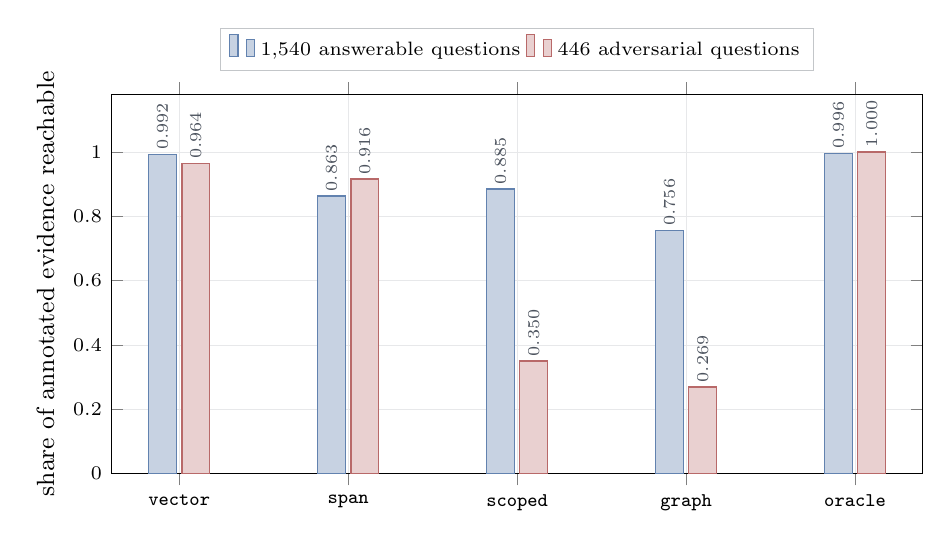
\begin{tikzpicture}
\begin{axis}[
  width=0.98\linewidth, height=6.4cm,
  ybar=2pt, bar width=10pt,
  ymin=0, ymax=1.18,
  ylabel={share of annotated evidence reachable},
  symbolic x coords={vector, span, scoped, graph, oracle},
  xtick=data,
  ytick={0,0.2,0.4,0.6,0.8,1.0},
  tick label style={font=\scriptsize},
  xticklabel style={font=\scriptsize\ttfamily},
  label style={font=\small},
  grid=major, grid style={hzslate!12, line width=0.2pt},
  legend style={font=\scriptsize, at={(0.5,1.06)}, anchor=south,
                legend columns=2, draw=hzslate!30, fill=white},
  legend cell align=left,
  nodes near coords,
  every node near coord/.append style={font=\fontsize{6}{7}\selectfont,
    color=hzslate!90, rotate=90, anchor=west, inner sep=1.5pt,
    /pgf/number format/fixed, /pgf/number format/fixed zerofill,
    /pgf/number format/precision=3},
]
\addplot[draw=hzblue!70, fill=hzblue!25] coordinates {
  (vector,0.992) (span,0.863) (scoped,0.885) (graph,0.756) (oracle,0.996)};
\addlegendentry{1{,}540 answerable questions}
\addplot[draw=hzred!70, fill=hzred!22] coordinates {
  (vector,0.964) (span,0.916) (scoped,0.350) (graph,0.269) (oracle,1.000)};
\addlegendentry{446 adversarial questions}
\end{axis}
\end{tikzpicture}
\caption{What each index can return at all, with the result limit lifted past
the number of turns in the conversation ($k=2000$, no abstention). This is
reach, not ranking, and it owes nothing to the reader. The two flat indexes
reach almost every annotated turn of both kinds. Against \texttt{vector}, the
two subject-scoped indexes give up 11 and 24 points of the answerable evidence
and 61 and 70 points of the adversarial evidence: they are selectively blind,
and the blindness falls where the trap turns are. \texttt{oracle} is handed the
annotated evidence and is shown as the frame of the measurement.}
\label{fig:reach}
\end{figure}


\emph{Interpretation.} The subject restriction makes the index selectively
blind, and the blindness is concentrated where the trap turns are. Measured
against \arm{vector}, it costs $11$ points of answerable evidence on whole turns
and $24$ on claim spans, which is the price of a rule-based extractor: a
sentence whose subject it fails to resolve produces no span for that person, and
the turn becomes unreachable through them. It removes $61$ and $70$ points of
adversarial evidence, which is the point, because an adversarial question's
annotated evidence is a turn about somebody else.

Stated precisely: a flat index has no representation of what a question is
\emph{about}, only of what it says, and an adversarial question says almost
exactly what the trap turn says. Partitioning
the index by sentence subject gives the query a second criterion that the
distractor fails. Nothing about a graph is required for that. What is required
is that the index be partitioned by the same attribute the question names, and
that the partition be derivable from the text.

\section{Is the gain bought with silence?}
\label{sec:abstention}

Declining is worth a full point on an adversarial question and costs whatever
the answer was worth everywhere else, so a comparison at one abstention
threshold is arguable by construction. In Table~\ref{tab:main} \arm{graph} is
silent on $31\%$ of questions and \arm{vector} on $20\%$. Two measurements
settle whether that difference is the gain.

\subsection{The abstention decision carries information, or it does not}

Abstention here is a threshold on one number: the confidence, computed
identically for every system, that the returned evidence covers the question's
rare terms. Whether that number separates an answerable question from an
adversarial one is a property of the memory and is independent of where the
threshold is put. We measure it as the area under the ROC curve, equivalently
the Mann--Whitney statistic with mid-ranked ties~\cite{hanleymcneil,mannwhitney}:
the probability that a randomly chosen answerable question receives a higher
confidence than a randomly chosen adversarial one.

\begin{center}
\small
\begin{tabular}{@{}lcc@{}}
\toprule
system & indexed unit / reachable & AUC \\
\midrule
\arm{vector} & turn / everything          & 0.514 \\
\arm{span}   & span / everything          & 0.514 \\
\arm{scoped} & turn / the subject's       & 0.635 \\
\arm{graph}  & span / the subject's       & \textbf{0.698} \\
\arm{oracle} & the annotated evidence     & 0.503 \\
\bottomrule
\end{tabular}
\end{center}

Both flat indexes are at chance. Their confidence is high on an adversarial
question for the same reason it is high on a single-hop question --- a turn
close to the question's wording was found --- and that is the entire content of
the signal. Both subject-scoped indexes are above chance, and the AUC tracks the
scope factor, not the unit factor: changing the unit alone leaves it at chance,
$0.514$ either way, while adding the scope moves it by $0.120$ on turns and
$0.184$ on spans. The oracle is also at chance. Perfect retrieval confers no ability to tell an answerable
question from an unanswerable one, because an adversarial question does have
retrievable evidence and it is exactly the wrong evidence.

At the operating point of Table~\ref{tab:main}, the realised binary decision has
AUC $0.627$ for \arm{graph} (declining on $50.2\%$ of adversarial and $24.9\%$
of answerable questions) and $0.500$ for \arm{vector} ($20.0\%$ and $20.0\%$).
The flat index declines at the same rate on both halves because it cannot tell
them apart.

\subsection{The whole trade, swept}

\begin{figure}[t]
\centering
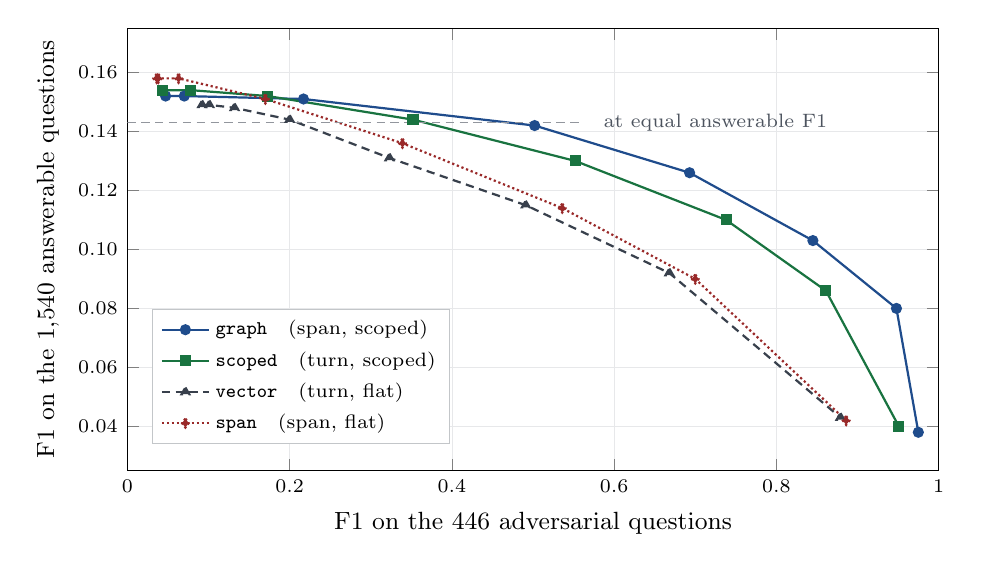
\begin{tikzpicture}
\begin{axis}[
  width=0.98\linewidth, height=7.2cm,
  xlabel={F1 on the 446 adversarial questions},
  ylabel={F1 on the 1{,}540 answerable questions},
  xmin=0, xmax=1.0, ymin=0.025, ymax=0.175,
  xtick={0,0.2,0.4,0.6,0.8,1.0},
  ytick={0.04,0.06,0.08,0.10,0.12,0.14,0.16},
  grid=both, grid style={hzslate!12, line width=0.2pt},
  scaled y ticks=false,
  y tick label style={/pgf/number format/fixed,
                      /pgf/number format/fixed zerofill,
                      /pgf/number format/precision=2},
  tick label style={font=\scriptsize},
  label style={font=\small},
  legend style={font=\scriptsize, at={(0.03,0.06)}, anchor=south west,
                draw=hzslate!30, fill=white, row sep=0.5pt},
  legend cell align=left,
  every axis plot/.append style={line width=0.8pt, mark size=1.6pt},
]

% floor = 0, 0.1, 0.2, 0.3, 0.4, 0.5, 0.6, 0.8
\addplot[hzblue, mark=*] coordinates {
  (0.047,0.152) (0.070,0.152) (0.217,0.151) (0.502,0.142)
  (0.693,0.126) (0.845,0.103) (0.948,0.080) (0.975,0.038)};
\addlegendentry{\texttt{graph} \; (span, scoped)}

\addplot[hzgreen, mark=square*] coordinates {
  (0.043,0.154) (0.078,0.154) (0.173,0.152) (0.352,0.144)
  (0.552,0.130) (0.738,0.110) (0.861,0.086) (0.951,0.040)};
\addlegendentry{\texttt{scoped} \; (turn, scoped)}

\addplot[hzslate, mark=triangle*, densely dashed] coordinates {
  (0.092,0.149) (0.101,0.149) (0.132,0.148) (0.200,0.144)
  (0.323,0.131) (0.491,0.115) (0.668,0.092) (0.879,0.043)};
\addlegendentry{\texttt{vector} \; (turn, flat)}

\addplot[hzred, mark=diamond*, densely dotted] coordinates {
  (0.036,0.158) (0.038,0.158) (0.063,0.158) (0.170,0.151)
  (0.339,0.136) (0.536,0.114) (0.700,0.090) (0.886,0.042)};
\addlegendentry{\texttt{span} \; (span, flat)}

\draw[hzslate!55, line width=0.3pt, densely dashed]
  (axis cs:0.0,0.143) -- (axis cs:0.56,0.143);
\node[font=\scriptsize, color=hzslate!90, anchor=west]
  at (axis cs:0.575,0.143) {at equal answerable F1};
\end{axis}
\end{tikzpicture}
\caption{The trade each index can make, swept over the abstention threshold
(\texttt{floor} $=0,\,0.1,\,0.2,\,0.3,\,0.4,\,0.5,\,0.6,\,0.8$; the marked
point fourth from the left on each curve is the operating point of
Table~\ref{tab:main}). These are four curves, not four points on one curve. At
the answerable F1 the arms all sit near ($y \approx 0.143$, dashed), the
subject-scoped indexes reach $0.502$ and $0.352$ on the adversarial questions
where the flat ones reach $0.200$ and $0.170$.}
\label{fig:frontier}
\end{figure}


Sweeping the abstention floor traces what each index can achieve, and
Figure~\ref{fig:frontier} plots the answerable score against the adversarial
score along that sweep. The four systems lie on four curves, not on one. At any
answerable score the two subject-scoped indexes are far to the right of the two
flat ones.

Matching the systems on silence rather than on threshold gives the same answer
in the units the objection is usually raised in. Reading each system at whichever
floor makes it as quiet as the other:

\begin{center}
\small
\begin{tabular}{@{}lrrrr@{}}
\toprule
silence & \arm{graph} answerable & \arm{graph} adversarial
        & \arm{vector} answerable & \arm{vector} adversarial \\
\midrule
$\approx$12\% & 0.151 & 0.217 & 0.148 & 0.132 \\
$\approx$32\% & 0.142 & 0.502 & 0.131 & 0.323 \\
$\approx$48\% & 0.126 & 0.693 & 0.115 & 0.491 \\
$\approx$62\% & 0.103 & 0.845 & 0.092 & 0.668 \\
\bottomrule
\end{tabular}
\end{center}

At each of the four matched rates \arm{graph} leads on both halves. The lead
belongs to the middle of the range rather than to all of it. Matched at $8\%$
silence --- \arm{vector} declines no less often than that, even with the floor
at zero --- the adversarial scores are $0.094$ against $0.092$, a gap inside the
between-conversation variation of Table~\ref{tab:ci}, and below that rate
\arm{vector} cannot be matched at all. Either system can be made as quiet
as one likes; over the range where declining is worth anything, only one of them
falls silent on the right questions.

\section{Perfect retrieval is a liability on unanswerable questions}
\label{sec:oracle}

The \arm{oracle} system is handed the turns the dataset itself annotates as the
evidence for each question. It is in the tables to bound the reader, and it also
produces an inversion worth reporting on its own.

On answerable questions the oracle is the best system, as it must be: $0.202$
against $0.142$ and $0.144$, and $0.306$ with abstention off. On adversarial
questions it scores $0.426$, \emph{below} \arm{graph}'s $0.502$, and with
abstention off it scores $0.045$, below even \arm{vector}'s $0.092$.

The reason is structural rather than incidental. An adversarial question in
LoCoMo has annotated evidence, and that evidence is the trap turn: the turn
where the other speaker described the activity. Handing a system that turn is
handing it exactly the material out of which a confident wrong answer is built.
Retrieval quality and answer quality diverge here --- the system retrieves the
right turn and answers the wrong question.

This has a consequence for evaluation beyond this benchmark. Retrieval metrics
computed against annotated evidence --- recall@$k$, MRR, nDCG --- reward finding
the annotated turn for every question in the set. On a set containing
unanswerable questions with annotated distractors, that reward is inverted for
part of the set, and a retriever tuned on it is tuned partly in the wrong
direction. We measured this on one benchmark and state it as an observation
about that benchmark; whether it generalises is an open question and
\S\ref{sec:settle} says what would answer it.

\section{Negative controls}
\label{sec:controls}

A negative control is an intervention that should change the outcome if the
proposed mechanism is the real one, and leaves it alone
otherwise~\cite{negativecontrol}. The system under test is described as a graph
memory with an inference layer. Three controls ask whether either is doing
anything.

\subsection{The graph}
\label{sec:control-graph}

\textbf{Intervention:} construct the knowledge graph from the empty fact set
instead of from the 23{,}942 extracted claims --- zero nodes, zero edges --- and
change nothing else.

\textbf{Result:} every figure in Tables~\ref{tab:main} and \ref{tab:factorial}
is byte-identical, and so is every bar of Figure~\ref{fig:reach}.

The graph is where the read turns are kept; it is not what answers a question.
Retrieval is cosine similarity through the store, and the store is populated
from the claims directly. The graph object is consulted only to report how many
nodes and edges were built. We had described this system as answering by ``a
lookup on a node rather than a nearest neighbour''; that description was false,
and this control is what falsified it.

\subsection{Inference}
\label{sec:control-reason}

\textbf{Intervention:} delete the derived facts entirely --- run no inference,
index nothing the reasoner produced.

\textbf{Result:} nothing moves by more than two thousandths, and what moves goes
both ways. Single-hop F1 rises from $0.121$ to $0.122$, while reach falls
wherever the graph's index is read --- single hop $0.507$ to $0.505$, answerable
$0.444$ to $0.443$, overall $0.375$ to $0.374$, in the \arm{graph} and
\arm{graph+edge} columns alike --- and \arm{graph+edge} declines on $22\%$ of
single-hop questions rather than $21\%$. No F1 on either half moves at three
decimals: answerable is $0.142$ either way, adversarial $0.502$, the aggregate
$0.223$. The 44 derived facts are worth two thousandths of single-hop reach, and
that reach does not become an answer.

The engine runs one rule --- what a thing is called is also what its owner has,
so ``I have a snake named Susie'' answers a question about the snake's name ---
to closure depth one, and derives 44 facts from 23{,}942 claims. That ratio is
the finding rather than the rule's weakness. Conversational memory is dominated
by aggregation over identity: the same person mentioned in two sessions is one
key --- here the folded name each indexed piece is filed under, which
\S\ref{sec:control-graph} showed is what retrieval actually reads --- and that
requires no inference at all. Once identity is resolved there is very little for
a reasoner to add. This says where the value in a memory graph sits, and it is
not in the deductive layer.

\subsection{The claim-span unit, and where the effect actually is}
\label{sec:factorial}

The remaining explanation has two parts, and Table~\ref{tab:factorial} separates
them by running all four cells of \S\ref{sec:indexes}.

\begin{table}[t]
\centering
\small
\caption{The $2\times2$ over indexed unit and reachable set, on the 446
adversarial questions and the 1{,}540 answerable ones. Effects are differences
in F1 computed from the unrounded scores (\S\ref{sec:metric}); the interaction
is $(\arm{graph}-\arm{scoped})-(\arm{span}-\arm{vector})$.}
\label{tab:factorial}
\begin{tabular}{@{}l cc c cc@{}}
\toprule
& \multicolumn{2}{c}{adversarial F1} & & \multicolumn{2}{c}{answerable F1} \\
\cmidrule(lr){2-3}\cmidrule(lr){5-6}
indexed unit & all reachable & subject's only & & all reachable & subject's only \\
\midrule
whole turn & 0.200 & 0.352 & & 0.144 & 0.144 \\
claim span & 0.170 & \textbf{0.502} & & 0.151 & 0.142 \\
\midrule
\multicolumn{6}{@{}l}{\emph{simple effects, adversarial}} \\
\multicolumn{6}{@{}l}{\quad subject scope, on whole turns \hfill $+0.152$} \\
\multicolumn{6}{@{}l}{\quad subject scope, on claim spans \hfill $+0.332$} \\
\multicolumn{6}{@{}l}{\quad claim span, with everything reachable \hfill $-0.029$} \\
\multicolumn{6}{@{}l}{\quad claim span, with scope in place \hfill $+0.150$} \\
\multicolumn{6}{@{}l}{\emph{main effects and interaction, adversarial}} \\
\multicolumn{6}{@{}l}{\quad subject scope \hfill $+0.242$} \\
\multicolumn{6}{@{}l}{\quad claim span \hfill $+0.061$} \\
\multicolumn{6}{@{}l}{\quad interaction \hfill $+0.179$} \\
\bottomrule
\end{tabular}
\end{table}

Three statements follow, all measured, with intervals in Table~\ref{tab:ci}.

\textbf{Subject scope on the unchanged turn index accounts for half the
effect.} Adding nothing but the subject partition to the turn index takes the
adversarial score from $0.200$ to $0.352$: a simple effect of $+0.152$ against
a total of $+0.303$, with no movement on the answerable half ($0.144$ to
$0.144$). Averaged over both units the main effect of the same partition is
larger, $+0.242$, because it is worth more on claim spans than on turns;
Table~\ref{tab:factorial} reports both and they are not interchangeable. No
claim extraction is needed to index by subject --- the extractor is used here
only to decide which people a turn is about --- and no graph is needed at all.

\textbf{The claim-span unit alone is harmful.} With everything still reachable,
narrowing the indexed unit takes the adversarial score \emph{down}, from
$0.200$ to $0.170$, and the interval excludes zero. The reason is visible in
Figure~\ref{fig:reach}: the flat span index reaches slightly less adversarial
evidence than the flat turn index in total ($0.916$ against $0.964$) but ranks
it much higher, returning $0.571$ of it in the top five against the turn
index's $0.511$. A short span consisting only of the sentence about yoga
matches a question about yoga better than a whole turn does. Sharpening the match without restricting
what may be matched just makes the trap easier to find.

\textbf{The largest single term is the interaction.} $+0.179$ of the $+0.303$
belongs to neither factor alone. Narrowing the unit is what makes the partition
sharp: a whole turn belongs to every person spoken of within it, so scoping
whole turns still admits the trap turn whenever both speakers appear in it,
while a claim span belongs to exactly one person. The worked example of
\S\ref{sec:result} is one case of it: \texttt{D20:2} congratulates Tim and then
reports John's own yoga, so the whole turn is filed under both, and \arm{scoped}
retrieves it for the question about Tim and answers \emph{yoga} exactly as
\arm{vector} does. Only the sentence-level unit keeps it out of Tim's pieces. The two changes are not
independent contributions to be added; the second is what makes the first work.

So the honest description of the system is not ``a graph memory'' and not ``an
extractive claim index''. It is: \emph{an index partitioned by the subject of
each sentence, queried by the subject of the question, at a granularity fine
enough that the partition is unambiguous.}

\section{Where subject scope does not help}
\label{sec:where-not}

\paragraph{Multi-hop, which was the expectation.} A graph memory is supposed to
help most where one person's several answers were given months apart and are
one node's several edges. Retrieval bears that out slightly: \arm{graph}'s
multi-hop reach is $0.228$ against \arm{vector}'s $0.194$ at $k=5$, and $0.419$
against $0.388$ under settings that let an answer be a list, which
\S\ref{sec:repro} names. F1 does not follow: $0.020$ against
$0.023$, and $0.053$ against $0.057$. Gathering the turns is not the hard part
of a multi-hop answer; assembling four phrases from four sessions into one list
is, and an extractive reader cannot. The oracle scores $0.068$ with perfect
evidence, which is the ceiling this reader puts on the category, so the
comparison here is close to uninformative and we do not draw a conclusion from
it.

There is a second caveat, and it qualifies our own earlier
work~\cite{multihop}, which proposed cross-session entity linkage as the
missing signal for multi-hop retrieval. We built that linkage, and at unbounded
$k$ \arm{graph} reaches $0.688$ of multi-hop evidence where \arm{vector} reaches
$0.985$. Subject scope improves multi-hop \emph{ranking} at small $k$
and lowers the \emph{ceiling} on what can be recovered at any $k$, because a
multi-hop question's evidence is not all filed under one person. Whether a
linkage that keeps everything reachable would help is untested here.

\paragraph{Answering off an edge.} \arm{graph+edge} reads the answer from the
matched edge --- the object phrase the extractor produced --- instead of quoting
the turn. It is worse on single-hop by more than half, $0.056$ against $0.121$.
The extracted object is a lossy paraphrase, and the sentence is what the
reference answer was written from. The graph is a better index than it is a
store of answers, at least when the extractor is rules rather than a model.

\paragraph{Open-domain.} All four systems score between $0.016$ and $0.018$,
and the oracle scores $0.032$. The category asks for an inference beyond what
was said, which the reader cannot make from any evidence. Nothing is measurable
here.

\section{Related work}
\label{sec:related}

LoCoMo~\cite{locomo} established the long-horizon conversational memory task and
supplies the per-question evidence annotations that make reach computable at
all. Its adversarial category follows the design of SQuAD~2.0's unanswerable
questions~\cite{squad2}: a plausible distractor present in the context, with
abstention as the correct response. Our \S\ref{sec:degenerate} is a caution
about aggregating over such a category rather than a criticism of including it;
including it is the right design, and averaging over it is not.

Retrieval-augmented generation~\cite{rag} over dense
passage retrieval~\cite{dpr} is the construction the flat baseline stands in
for, with a lexical weighting substituted for a learned embedding for the
reasons given in \S\ref{sec:indexes}. That weighting is term frequency times
inverse document frequency at unit length, compared by cosine, and not
BM25~\cite{bm25}; BM25's saturation and length terms would make the baseline
stronger still, so \S\ref{sec:indexes}'s argument that the lexical arm is the
harder one does not rest on the strongest form of it. Graph-structured and
entity-structured memory --- GraphRAG~\cite{graphrag}, HippoRAG~\cite{hipporag},
MemGPT~\cite{memgpt} --- is the family the system under test belongs to. Our
contribution to that line is a decomposition rather than a system: of the
components such a construction bundles together, we find that on this benchmark
the graph and the inference layer contribute nothing
measurable, and the partition of the index by entity accounts for the whole of
the measured effect. That is consistent with
those systems working, and inconsistent with the graph being why.

Our earlier measurement on this corpus~\cite{multihop} showed that repeated
retrieval does not fix multi-hop questions and named cross-session entity
linkage as the missing signal. \S\ref{sec:where-not} reports that we built the
linkage and multi-hop F1 did not move, with the reader ceiling as a confound
and a reduction in reach as a real cost. That is a partial qualification of the
earlier proposal, not a refutation of it.

Methodologically the paper is an instance of a standing argument in empirical
retrieval and representation learning: that improvements attributed to an
elaborate mechanism frequently survive its removal, and that the fix is
stronger baselines and complete ablations~\cite{neuralhype,realitycheck}. The
negative-control framing is borrowed from epidemiology~\cite{negativecontrol},
where an intervention that should move the outcome and does not is treated as
evidence about the mechanism rather than as a null finding to be discarded.

\section{Limitations}
\label{sec:limits}

\textbf{No model reader.} This is the largest limitation and it bounds every
other claim. The oracle reaches $0.306$ on answerable questions with perfect
retrieval, so the answerable column compresses a wide range of retrieval quality
into a narrow range of F1. ``No cost on answerable questions'' means ``no cost
this reader can detect'', and \S\ref{sec:mechanism} shows a real cost in reach
($0.756$ against $0.992$) that a stronger reader would very likely convert into
a real cost in F1. The direction of the adversarial result is unlikely to
reverse --- it rests on evidence never being retrieved, not on the reader ---
but its magnitude relative to a cost on the answerable half is not established.

\textbf{Ten conversations.} The intervals in Table~\ref{tab:ci} are bootstrapped
over ten units, which is a small number of units for a percentile interval. They
should be read as indicating that the adversarial effect is large relative to
between-conversation variation, not as precise coverage statements.

\textbf{One dataset, one language, synthetic dialogue.} LoCoMo is generated and
then verified, two-party, and English. The subject-resolution rule that carries
the extraction --- \emph{I} is the speaker, \emph{you} is the other party ---
is a two-party rule and does not survive a group conversation unmodified.
$98.9\%$ of questions naming a speaker is a property of this question set.

\textbf{Lexical retrieval.} We argue in \S\ref{sec:indexes} that lexical
weighting is the harder baseline on this corpus and give the reason, but it is
an argument, not a measurement. The subject-scoping result is a claim about what
is indexed and should transfer to a dense index; that it does transfer is
untested.

\textbf{A rule-based extractor.} The $11$ and $24$ points of answerable reach
the two subject-scoped indexes give up are the extractor's failures, not a
property of subject scoping. A model-based extractor would move that cost and we
do not know by how much.

\section{What would settle it}
\label{sec:settle}

Four experiments, in the order we would run them.

\begin{enumerate}[leftmargin=1.4em,itemsep=3pt]
\item \textbf{A model reader behind both indexes, unchanged otherwise.} This
      removes the ceiling of \S\ref{sec:reader}, and it is what would show
      whether the reach cost of subject scoping is a real cost in answers. It
      turns the comparison into a comparison of two prompts as well as two
      indexes, so both arms must share one prompt verbatim, with the retrieved
      evidence the only difference.

\item \textbf{Subject scoping over a dense retriever.} Take an embedding index,
      attach the subject partition as a metadata filter, and change nothing
      else. The claim in \S\ref{sec:mechanism} is that the effect is a property
      of what is indexed and not of how vectors are made; this is the experiment
      that would falsify it. A dense index on this exact corpus already exists
      in-house~\cite{multihop}.

\item \textbf{A second dataset with annotated unanswerable questions.} The
      oracle inversion of \S\ref{sec:oracle} --- perfect retrieval scoring worse
      where the annotated evidence is the distractor --- is an observation about
      LoCoMo. Reproducing it on an independent benchmark would make it a
      statement about evaluation design rather than about one dataset.

\item \textbf{A model-based extractor for the subject partition.} If it recovers
      the answerable reach the rule-based extractor loses while keeping the
      adversarial blindness, then subject scoping costs nothing and the case for
      it is complete. If it recovers the adversarial reach too, then the
      blindness was the extractor's failures all along, and the result in this
      paper is an accident of a weak extractor. We consider the second outcome
      unlikely, since \arm{scoped} and \arm{graph} lose adversarial reach in
      proportion to how sharply the partition is defined rather than in
      proportion to extraction errors, but it is not ruled out by anything here.
\end{enumerate}

\section{Reproducibility}
\label{sec:repro}

The harness is \texttt{bench/locomo/} in \texttt{hanzoai/semantic}~\cite{semantic},
MIT, tag \texttt{v0.2.4}. It is Go with no dependencies outside the standard
library and that repository, and it fetches the dataset itself on first run
(2{,}805{,}274 bytes, SHA-256
\texttt{79fa87e9\ldots ea698ff4}, from the LoCoMo GitHub repository rather than
the Hugging Face mirror, which holds no data). Neither the dataset nor the
original \texttt{evaluation.py} is redistributed: LoCoMo is CC BY-NC 4.0 and the
harness is MIT, so both are fetched at run time.

Every figure in this paper is produced by one of the following, run from the
repository root. The first group is \texttt{go run ./bench/locomo} with the
flags shown:

\begin{center}
\footnotesize
\begin{tabular}{@{}ll@{}}
\toprule
flags & what it produces \\
\midrule
(none) & Table~\ref{tab:main}; the corpus, build and subject counts of \S\ref{sec:setup} \\
\texttt{-factor} & Table~\ref{tab:factorial} \\
\texttt{-sweep floor} & Figure~\ref{fig:frontier}, the matched-silence table of \S\ref{sec:abstention} \\
\texttt{-sweep span} (also \texttt{band}, \texttt{parts}) & the reader settings of \S\ref{sec:reader} \\
\texttt{-k 2000 -floor 0} & Figure~\ref{fig:reach}, \S\ref{sec:mechanism}, the unbounded-$k$ reach of \S\ref{sec:where-not} \\
\texttt{-k 20 -parts 4 -band 0.5} & the multi-hop list figures of \S\ref{sec:where-not} \\
\texttt{-floor 0.13} & the low-silence crossing of \S\ref{sec:abstention} \\
\texttt{-out <file>} & the per-question record \\
\texttt{-stats <file>} & \S\ref{sec:degenerate}, the AUCs of \S\ref{sec:abstention}, Table~\ref{tab:ci} \\
\midrule
\multicolumn{2}{@{}l}{\emph{and, as whole commands:}} \\
\texttt{make golden} \emph{(in \texttt{bench/locomo})} & the two golden files the metric tests read \\
\texttt{go test -v ./bench/locomo/} & the metric port, three ways, with the counts of \S\ref{sec:metric} \\
\texttt{make check} \emph{(in \texttt{bench/locomo})} & Tables~\ref{tab:main} and \ref{tab:factorial}, by the original Python \\
\bottomrule
\end{tabular}
\end{center}

Every row in the first group also takes \texttt{-factor}, which swaps
\arm{graph+edge} and \arm{oracle} for \arm{scoped} and \arm{span};
Figures~\ref{fig:reach} and \ref{fig:frontier} are drawn from both arm sets.
\texttt{-stats} reads a predictions file back rather than the memories: the file
carries each system's reply, its retrieved turn identifiers and its confidence,
so the constant-abstention score of \S\ref{sec:degenerate}, the AUCs of
\S\ref{sec:abstention} and the intervals of Table~\ref{tab:ci} are computed from
a published artifact rather than asserted beside it. Two of the three golden
files quote the dataset and so are not kept in the repository; the tests that
read them skip until \texttt{make golden} has written them.

Four things come from outside that table. The dataset's length and digest are of
the file the harness fetches, read with \texttt{shasum -a 256}; the shape of the
adversarial questions in \S\ref{sec:setup} --- which fields they carry, and what
is in them --- is read off that same file. The cost in \S\ref{sec:indexes} is
\texttt{/usr/bin/time -l} over the built binary. And the two controls of
\S\ref{sec:control-graph} and \S\ref{sec:control-reason} are single-line edits
to \texttt{graph.go} --- build the graph from the empty fact set, and skip the
loop over the derived facts --- after which the first row of the table reports
what changed.

\section{Conclusion}
\label{sec:conclusion}

Three findings, of which only the last is of the kind usually reported.

The aggregate that would ordinarily be quoted for this benchmark is degenerate.
Constant abstention scores $0.228$, above every system here that has to find its
own evidence and within $0.024$ of one handed the annotated evidence. Any mean
over a question set in which a quarter of the questions reward silence measures
the abstention policy first.

The mechanism the system is named for is inert. Emptying the knowledge graph
leaves every figure byte-identical, and removing the inference layer, which
derived 44 facts from 23{,}942, moves no score on either half of the benchmark
and no figure anywhere by more than two thousandths. Neither of those is a
defect in the implementation; both say where the value in this kind of memory is
not.

What is left is worth stating exactly. Partitioning a retrieval index by the
subject of each sentence, and querying it with the subject of the question,
scores $0.502$ against $0.200$ on 446 adversarial questions with no cost this
reader can measure on 1{,}540 answerable ones, and it does so by making the
index unable to reach the trap turn: $27\%$ of adversarial evidence reachable
against $96\%$. Half of that gain is the partition applied to the unchanged
baseline; the claim-span unit on its own makes things worse; the largest single
term is their interaction, because a fine-grained unit is what makes the
partition unambiguous. An oracle with perfect retrieval does worse than
\arm{graph} on those questions, because there the right turn is the wrong
answer.

The useful part of this is the shape of the intervention, which is small.
Scoping retrieval to the entity a question names requires an attribute on each
indexed item and a filter on each query. It requires no graph, no inference, and
no change to the retrieval model. Whether it survives a model reader and a dense
index is the next measurement, and \S\ref{sec:settle} names it.

{\small
\bibliographystyle{plain}
\bibliography{references}
}

\end{document}
